\documentclass[tikz]{standalone}
\usepackage{bm}
\newcommand{\vect}{\bm}
\newcommand{\del}{\nabla}

\begin{document}
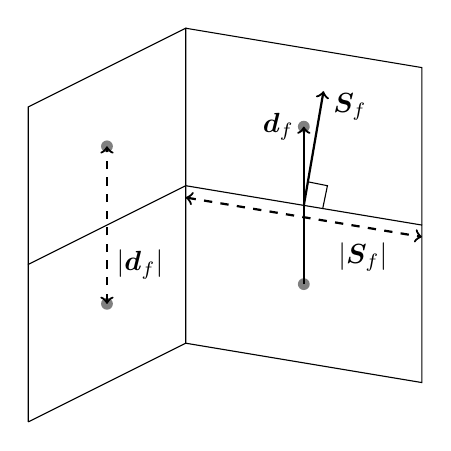
\begin{tikzpicture}[
  scale=0.5,
  cpnt/.style={fill=gray},
  arr/.style={thick, ->},
  mag/.style={dashed, thick, <->}
]
\draw (0,0) --  (4,2)  -- (4,6)  -- (0,4) -- (0,0);
\draw (4,2) --  (10,1) -- (10,5) -- (4,6);
\draw (0,4) --  (0,8)  -- (4,10)  -- (4,6);
\draw (10,5) -- (10,9) -- (4,10);
\path [cpnt] (2,3) circle [radius=0.15];
\path [cpnt] (2,7) circle [radius=0.15];
\path [cpnt] (7,3.5) circle [radius=0.15];
\path [cpnt] (7,7.5) circle [radius=0.15];
\draw [arr] (7,3.5) -- (7,7.5);
\draw [arr] (7,5.5) -- (7.5,8.4);
\node [left] at (7,7.5) {$\vect{d}_f$};
\node [right] at (7.5,8) {$\vect{S}_f$};
\draw [mag] (2,3) -- (2,7);
\node [right] at (2,4) {$|{\vect{d}_f}|$};
\draw [mag] (4,5.7) -- (10,4.7);
\node [below] at (8.5,4.8) {$|{\vect{S}_f}|$};
\draw (7.48,5.42) -- (7.6,6) -- (7.1,6.1);
\end{tikzpicture}
\end{document}
